\documentclass{beamer}
\usetheme{Rochester}
\usecolortheme{beaver}
\beamertemplatenavigationsymbolsempty
\usepackage{listings}
\lstset{basicstyle=\ttfamily}
\title{HTSQL}
\subtitle{A Database Query Language}
\begin{document}

\begin{frame}[plain]

\includegraphics[width=\textwidth]{img/rabbit-htsql.png}
\begin{center}
\texttt{http://htsql.org/}
\end{center}
\end{frame}

\begin{frame}
\frametitle{HTSQL --- A Database Query Language}
\textbf{\Large HTSQL is a comprehensive navigational query language for relational
databases.}

\bigskip
HTSQL is designed for data analysts and other \emph{accidental programmers} who
have complex business inquiries to solve and need a productive tool to write
and share database queries.

\bigskip
HTSQL is \emph{free and open source} software.
\end{frame}

\begin{frame}[containsverbatim]
\frametitle{An Example}
HTSQL directly maps common business inquiries onto a syntax parsable
and excutable by a computer.
\begin{columns}[c]
\begin{column}[T]{.5\textwidth}
\begin{block}{A business inquiry}
Show me for each school:
\begin{itemize}
\item its name, its location,
\item number of programs and departments,
\item and the average number of courses
      across each of its departments?
\end{itemize}
\end{block}
\end{column}
\begin{column}[T]{.5\textwidth}
\begin{block}{Translation to HTSQL}
\begin{lstlisting}
/school{
    name, campus,
    count(program),
    count(department),
    avg(department.
      count(course))}
\end{lstlisting}
\end{block}
\end{column}
\end{columns}
\end{frame}

\begin{frame}
\frametitle{HTSQL License}
HTSQL is \emph{free software}.  We offer support services, feature development,
and sells license exceptions for use of HTSQL in combination with proprietary
databases.
\begin{itemize}
\item
For open source database systems (SQLite, PostgreSQL, and MySQL), HTSQL is
released as free software under the terms of the AGPLv3. We also offer HTSQL
with a non-free, but otherwise permissive license so that proprietary
applications may use HTSQL in combination with open source database systems.
\item
For proprietary database systems (Oracle and Microsoft SQL Server), we offer
HTSQL under an evaluation and a proprietary license.
\end{itemize}


\end{frame}

\begin{frame}[containsverbatim]
\frametitle{HTSQL is a Python Library}
\begin{block}{\texttt{>>> from htsql import HTSQL}}
\begin{lstlisting}
>>> demo = HTSQL("pgsql:///htsql_demo")
>>> rows = demo.produce("/school")
>>> for row in rows:
...     print row
...
school(code=u'art',
       name=u'School of Art & Design',
       campus=u'old')
[...]
\end{lstlisting}
\end{block}
Download and install from PyPI:
\begin{lstlisting}
$ pip install HTSQL
\end{lstlisting}
\end{frame}

\begin{frame}[containsverbatim]
\frametitle{HTSQL is a Relational Database Gateway}
HTSQL queries are translated to SQL.  HTSQL has backends for
\emph{SQLite, PostgreSQL, MySQL, Oracle, MS SQL Server}.
\begin{columns}[c]
\begin{column}[T]{.5\textwidth}
\begin{block}{An HTSQL query}
\begin{lstlisting}
/school
\end{lstlisting}
\end{block}
\end{column}
\begin{column}[T]{.5\textwidth}
\begin{block}{Translation to SQL}
\begin{lstlisting}
SELECT
    "school"."code",
    "school"."name",
    "school"."campus"
FROM "ad"."school"
ORDER BY 1 ASC
\end{lstlisting}
\end{block}
\end{column}
\end{columns}
\end{frame}

\begin{frame}[containsverbatim]
\frametitle{HTSQL is an Advanced Query Language}
HTSQL is a complete query language featuring automated linking, aggregation,
projections, filters, macros, a compositional syntax, and a full set of data
types \& functions.
\begin{columns}[c]
\begin{column}[T]{.5\textwidth}
\begin{block}{An HTSQL query}
\begin{lstlisting}
/school{
    name,
    count(program),
    count(department)}
\end{lstlisting}
\end{block}
\end{column}
\begin{column}[T]{.5\textwidth}
\begin{block}{Translation to SQL}
\fontsize{1}{1}
\begin{lstlisting}
SELECT "school"."name",
 COALESCE("program"."count", 0),
 COALESCE("department"."count", 0)
FROM "ad"."school"
LEFT OUTER JOIN
(SELECT COUNT(TRUE) AS "count",
        "program"."school_code"
 FROM "ad"."program"
 GROUP BY 2) AS "program" ON
  ("school"."code" = "program"."school_code")
LEFT OUTER JOIN
(SELECT COUNT(TRUE) AS "count",
        "department"."school_code"
 FROM "ad"."department"
 GROUP BY 2) AS "department" ON
  ("school"."code" = "department"."school_code")
ORDER BY "school"."code" ASC
\end{lstlisting}
\end{block}
\end{column}
\end{columns}
\end{frame}

\begin{frame}[containsverbatim]
\frametitle{HTSQL is a WSGI Web Service}
HTSQL is a web service that accepts queries as URLs, returning results
formatted as HTML, JSON, CSV or XML.  With HTSQL, databases can be accessed,
secured, cached, and integrated using standard web technologies.
\begin{columns}[c]
\begin{column}[T]{.5\textwidth}
\begin{block}{HTTP request}
\begin{lstlisting}
GET /school HTTP/1.1
\end{lstlisting}
\end{block}
\end{column}
\begin{column}[T]{.5\textwidth}
\begin{block}{HTTP response}
\tiny
\begin{lstlisting}
{
  "school": [
    {
      "code": "art",
      "name": "School of Art & Design",
      "campus": "old"
    },
    {
      "code": "bus",
      "name": "School of Business",
      "campus": "south"
    },
    [...]
  ]
}
\end{lstlisting}
\end{block}
\end{column}
\end{columns}
\end{frame}

\begin{frame}[containsverbatim]
\frametitle{HTSQL Syntax: Basics}
\begin{block}{Literal values}
\begin{lstlisting}
/{3.14159, 'Hello World!'}
\end{lstlisting}
\end{block}
\begin{block}{Algebraic \& predicate expressions}
\begin{lstlisting}
/{(3+4)*6, (7<13)&(1=0|1!=0)}
\end{lstlisting}
\end{block}
\begin{block}{Schema navigation}
\begin{lstlisting}
/school

/school.department
\end{lstlisting}
\end{block}
\end{frame}

\begin{frame}[containsverbatim]
\frametitle{HTSQL Syntax: Filtering, Sorting, \& Truncating}
\begin{block}{Filtering rows}
\begin{lstlisting}
/school?campus='south'

/school.filter(campus='south')
\end{lstlisting}
\end{block}
\begin{block}{Sorting rows}
\begin{lstlisting}
/school.sort(campus)
\end{lstlisting}
\end{block}
\begin{block}{Truncating rows}
\begin{lstlisting}
/school.limit(3)
\end{lstlisting}
\end{block}
\end{frame}

\begin{frame}[containsverbatim]
\frametitle{HTSQL Syntax: Selection}
\begin{block}{Selecting output columns}
\begin{lstlisting}
/school{name, campus}

/school{name,
        count(department) :as '# of Dept'}
\end{lstlisting}
\end{block}
\begin{block}{Calculated attributes}
\begin{lstlisting}
/school
  .define(num_dept:=count(department))
  {code, num_dept}?num_dept>3
\end{lstlisting}
\end{block}
\end{frame}

\begin{frame}[containsverbatim]
\frametitle{HTSQL Syntax: Aggregates \& Projections}
\begin{block}{Aggregates}
\begin{lstlisting}
/{count(department),
  avg(school.count(department))}

/department{name,
    max(course.credits),
    avg(course.credits)}?exists(course)
\end{lstlisting}
\end{block}
\begin{block}{Projections}
\begin{lstlisting}
/(school^campus){campus, count(school)}

/school{name, count(program^degree)}
\end{lstlisting}
\end{block}
\end{frame}

\begin{frame}[containsverbatim]
\frametitle{HTRAF Toolkit --- Embedding Data into HTML}
\begin{columns}[c]
\begin{column}[T]{.5\textwidth}
\begin{block}{Demo}
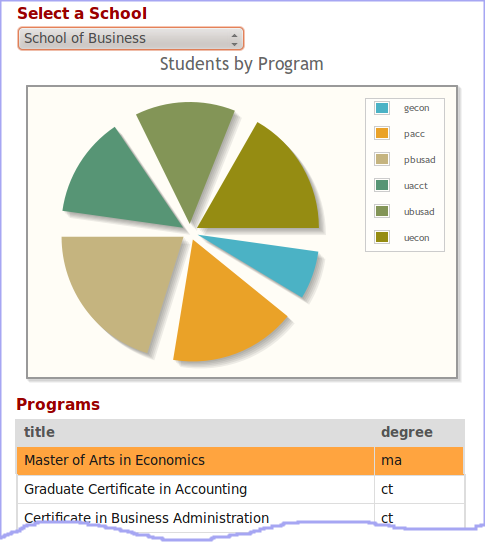
\includegraphics[width=\textwidth]{img/htraf-1.png}
\end{block}
\end{column}
\begin{column}[T]{.5\textwidth}
\begin{block}{HTML}
\tiny
\begin{lstlisting}
<h3>Select a School</h3>
<select id="school"
  data-htsql="/school{code, name}">
</select>

<div style="width: 400px;
            height: 350px;"
  data-htsql="/program{code,
                       count(student)}
                  ?exists(student)
                  &school.code=$school"
  data-ref="school"
  data-widget="chart"
  data-type="pie"
  data-title="Students by Program">
</div>

<h3>Programs</h3>
<table style="width: 400px"
  data-htsql="/program{title, degree}
                  ?school.code=$school"
  data-ref="school">
</table>
\end{lstlisting}
\end{block}
\end{column}
\end{columns}
\end{frame}

\begin{frame}[containsverbatim]
\frametitle{HTRAF: A Table Widget}
\begin{columns}[c]
\begin{column}[T]{.5\textwidth}
\begin{block}{HTML}
\small
\begin{lstlisting}
<table data-htsql=
    "/program{title,
              degree}">
</table>
\end{lstlisting}
\end{block}
\end{column}
\begin{column}[T]{.5\textwidth}
\begin{block}{Demo}
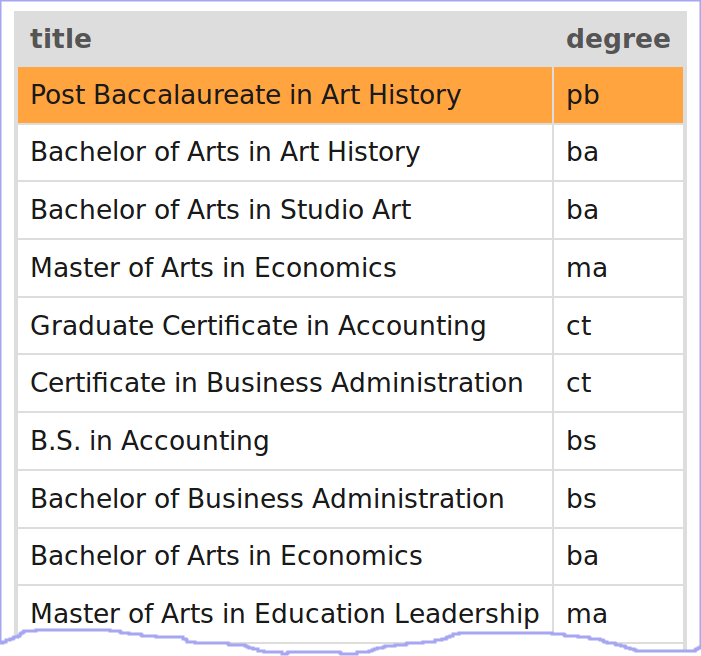
\includegraphics[width=\textwidth]{img/htraf-2.png}
\end{block}
\end{column}
\end{columns}
\end{frame}

\begin{frame}[containsverbatim]
\frametitle{HTRAF: A Chart Widget}
\begin{columns}[c]
\begin{column}[T]{.5\textwidth}
\begin{block}{HTML}
\small
\begin{lstlisting}
<div
  style="width: 450px;
         height: 350px;"
  data-htsql=
    "/program{
       code,
       count(student)}
      ?school.code='ns'"
  data-widget="chart"
  data-type="pie">
</div>
\end{lstlisting}
\end{block}
\end{column}
\begin{column}[T]{.5\textwidth}
\begin{block}{Demo}
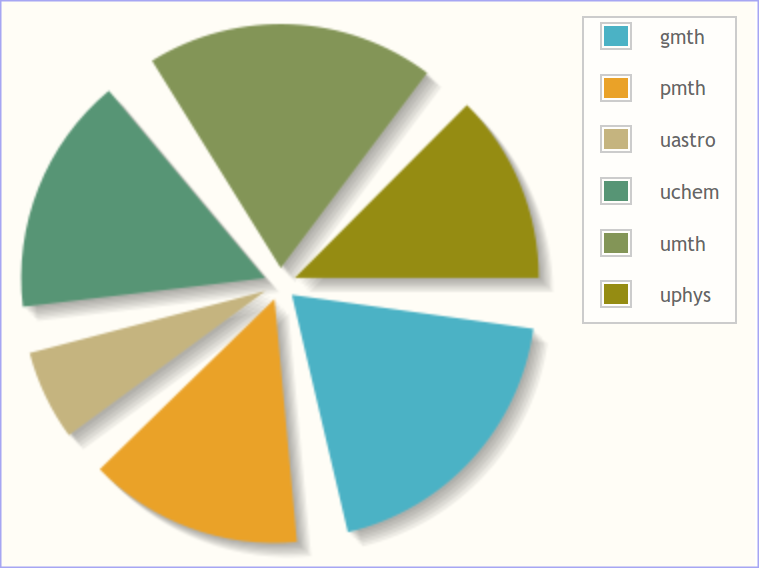
\includegraphics[width=\textwidth]{img/htraf-3.png}
\end{block}
\end{column}
\end{columns}
\end{frame}

\begin{frame}[containsverbatim]
\frametitle{HTRAF: Linking Widgets}
\begin{columns}[c]
\begin{column}[T]{.5\textwidth}
\begin{block}{HTML}
\small
\begin{lstlisting}
<select id="sc"
  data-htsql=
    "/school{code,
             name}">
</select>

<table
  data-htsql=
    "/program{title,
              degree}
      ?school.code=$sc"
  data-ref="sc">
</table>
\end{lstlisting}
\end{block}
\end{column}
\begin{column}[T]{.5\textwidth}
\begin{block}{Demo}
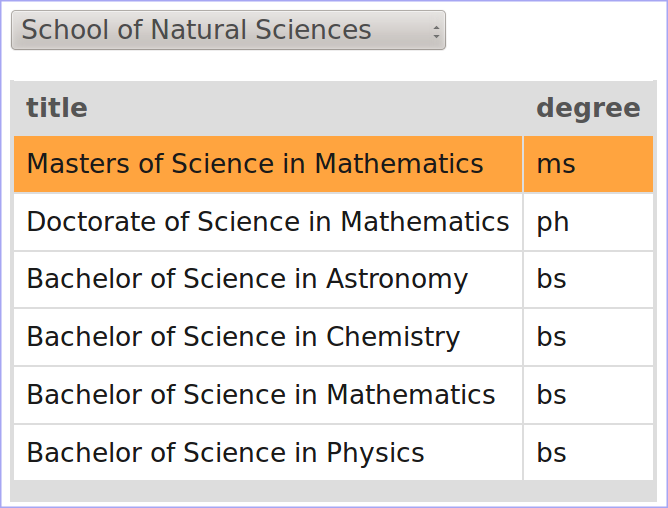
\includegraphics[width=\textwidth]{img/htraf-4.png}
\end{block}
\end{column}
\end{columns}
\end{frame}

\end{document}
